\subsection{Three Distillation Patterns of \ourmodel}
\label{rq5_body}
During training, \ourmodel exhibits three characteristic distillation patterns, as illustrated in Figure~\ref{rq5}:









\textbf{(1) Stable Pattern.} The student remains closely aligned with the teacher, \ie the step-level divergence $d_k$ is low. Therefore, adaptive weights stay high, allowing full utilization of teacher supervision along the trajectory. In this regime, the optimization closely resembles sufficient distillation.
\textbf{(2) Erroneous Pattern.} Persistent deviations increase step-level divergence, often caused by incorrect intermediate reasoning or tool usage. Adaptive weights are progressively reduced, which suppresses potentially misleading supervision and stabilizes training under such corrupted states.
\textbf{(3) Recovery Pattern.} The student initially deviates but then recovers. Weights are attenuated during high-divergence steps and restored later, enabling effective guidance on corrected steps and preserving useful supervision after recovery. This behavior allows the model to avoid over-penalizing temporary errors while still benefiting from supervision once alignment is re-established.







We also provide further analysis, \ie the quantitative analysis of distillation pattern distribution according training steps in~\cref{app:futher_casestudy}.
Detailed examples are provided in~\Cref{app:casestudy}.


\begin{figure*}[t]
\centering
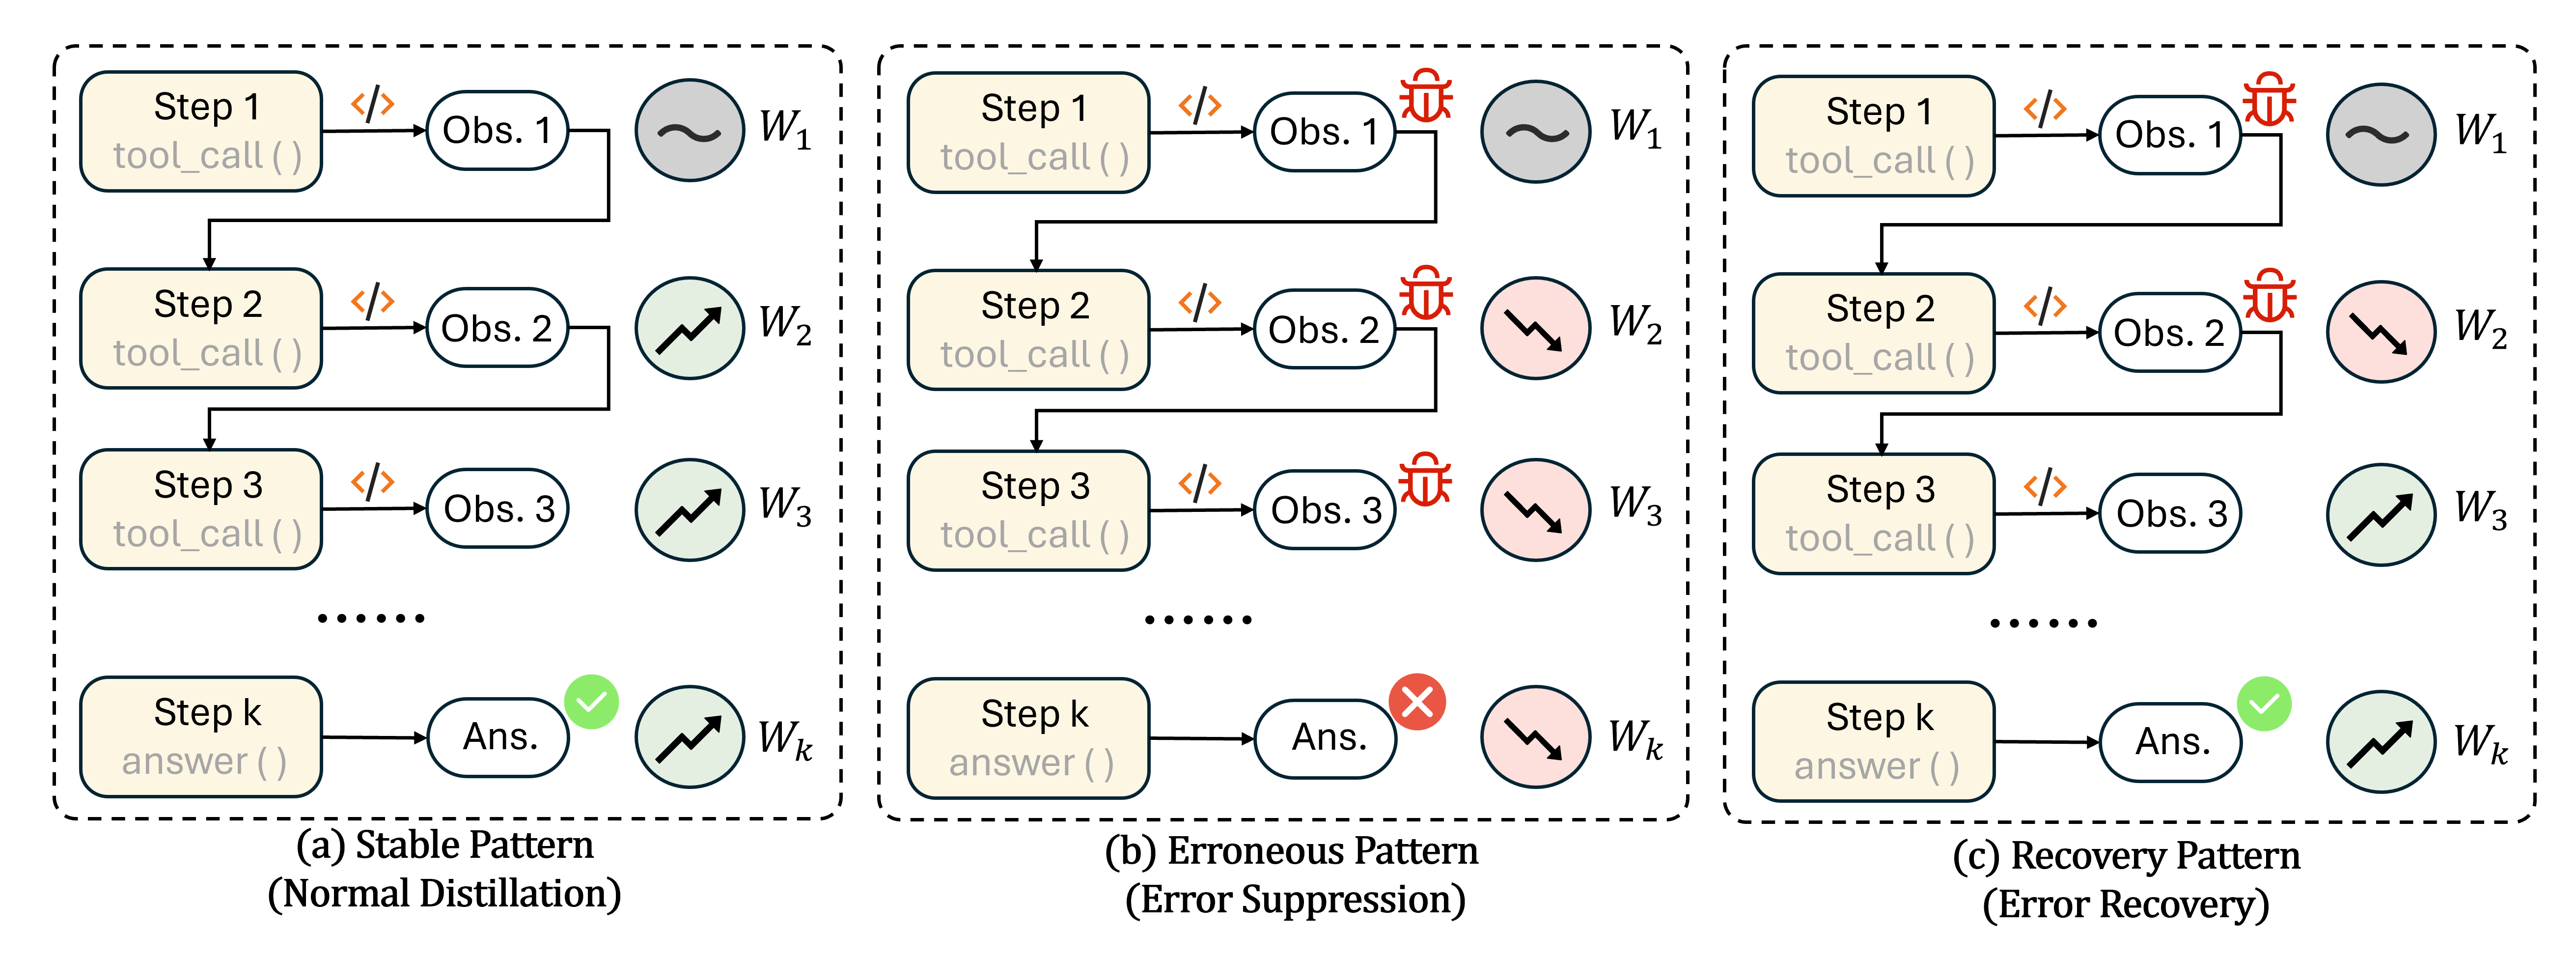
\includegraphics[width=1.0\linewidth]{pic/rq5_v5.png}
\caption{\textbf{Three distillation patterns of \ourmodel}.
}
\vspace{-1 em}
\label{rq5}
\end{figure*}
